%---------------------------------------------------------------------
% Course 	: Introduction To web sciences
% Professor : Dr.Nelson
% Name   	: Babitha Bokka
% Assignment: 5
%---------------------------------------------------------------------
\documentclass[12pt]{article}
%--------------------------------------------------------------------
% packages required
%--------------------------------------------------------------------
\usepackage{graphicx}
\usepackage{listings}
\usepackage{hyperref}
\usepackage{caption}
\usepackage{color}
\usepackage{pdfpages}
\graphicspath{ {images/} }
%--------------------------------------------------------------------
% Start Margins
%--------------------------------------------------------------------
\addtolength{\oddsidemargin}{-.875in}
\addtolength{\evensidemargin}{-.875in}
\addtolength{\textwidth}{1.75in}
\addtolength{\topmargin}{-.885in}
\addtolength{\textheight}{1.95in}
%-------------------------------------------------------------------
% End Margins
%--------------------------------------------------------------------
\definecolor{codegreen}{rgb}{0,0.6,0}
\definecolor{codegray}{rgb}{0.5,0.5,0.5}
\definecolor{codepurple}{rgb}{0.58,0,0.82}
\definecolor{backcolour}{rgb}{0.95,0.95,0.92}
 
\lstdefinestyle{mystyle}{
    backgroundcolor=\color{backcolour},   
    commentstyle=\color{codegreen},
    keywordstyle=\color{magenta},
    numberstyle=\tiny\color{codegray},
    stringstyle=\color{codepurple},
    basicstyle=\footnotesize,
    breakatwhitespace=false,         
    breaklines=true,                 
    captionpos=b,                    
    keepspaces=true,                 
    numbers=left,                    
    numbersep=5pt,                  
    showspaces=false,                
    showstringspaces=false,
    showtabs=false,                  
    tabsize=2
}
 
\lstset{style=mystyle}

\begin{document}

%---------------------------------------------------------------------
%Making the title page
%---------------------------------------------------------------------
\begin{titlepage}
\title{INTRODUCTION TO WEB SCIENCES:\\*Assignment 5}
\author{Babitha Bokka}
\date{17 October 2014}
\maketitle
\end{titlepage}

%---------------------------------------------------------------------
%Table of contents
%---------------------------------------------------------------------
\tableofcontents
\newpage
%------------------------------------------------------------------
%Question 1 (Twitter)
%------------------------------------------------------------------
\section{Question 1: Twitter Friendship Paradox}
Explore the friendship paradox for twitter account.
%-----------------------Approach----------------------------------
\subsection{Approach}
Intial step taken is looking for Tweepy Twitter API, found a good documentation to extract the friends (people you follow )from twitter account.Since my twitter account does not have more than 50 friends I used ``phonedude\_mln'' and extracted friends(whom phonedude\_mln follow ).
\subsection{Description of searchfriends.py}
\begin{enumerate}
	\item The program needs four Twitter API keys.
	\item Using the keys we interact with twitter API.
	\item Using the pre-defined methods we get the screen name and friend friends count.
	\item Saved the results to friendsCount.txt.
	\item Using the sort command sorted the friends count.
	\item Saved them to friendsCount.txt.sort.
\end{enumerate}

\subsection{Description of sortFriends.py}
\begin{enumerate}
	\item The sorted file is given as input to the program.
	\item The screen name (friends name) is given an ID and the ID and the count are saved to a file.
	\item To maintain a record which user is assigned which ID a log file numberNameCount.txt is created.
	\item The final friend ID and the count is saved to finalSorted.txt
\end{enumerate}
\newpage
%-----------------------Source Code-------------------------------
\subsection{Source Code}
\subsubsection{searchFriends.py}
\lstinputlisting[breaklines=True,language=Python]{../twitter/searchFriends.py}
\newpage

\subsubsection{sortingCommand.txt}
\lstinputlisting[breaklines=True,language=Python]{../twitter/sortingCommand.txt}

\subsubsection{sortFriends.py}
\lstinputlisting[breaklines=True,language=Python]{../twitter/sortFriends.py}
\newpage
%-----------------------Input Section---------------------------
\subsection{Input}
To accomplish the task ``phonedude\_mln'' twitter account is used.
%-----------------------Output Section---------------------------
\subsection{Output Files}
\subsubsection{friendsCount.txt}
The file contains the ``phonedude\_mln'' friends screen name and the count of their friends.
\lstinputlisting[breaklines=True]{../twitter/friendsCountfordoc.txt}

\subsubsection{friendsCount.txt.sort}
Sorting the friends based on the number of friends.
\lstinputlisting[breaklines=True]{../twitter/friendsCount.txt.sortfordoc}

\subsubsection{finalSorted.txt}
The file contains the friend ID and number of friends for each friend.
\lstinputlisting[breaklines=True]{../twitter/finalSortedfordoc.txt}

\subsubsection{numberNameCount.txt}
This is a log file which contains ID given to each friend, the count of friend friends, and screen name.
\lstinputlisting[breaklines=True]{../twitter/numberNameCountfordoc.txt}
\newpage


\subsection{Scatterplot}
\subsubsection{Code to generate the Scatterplot scatterCommands.txt}
\lstinputlisting[breaklines=True]{../twitter/scatterCommands.txt}
\subsubsection{Description of graph}
Figure 1 brings up the relation between the friends and number of friends. Figure 1 and Figure 2 are plotted on the same data but Figure 2 gives clear visualization.\\* 

\begin{figure}[ht]
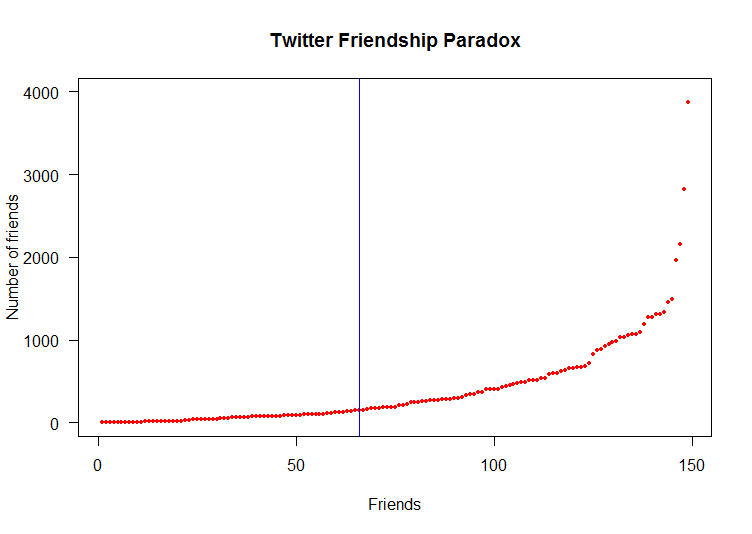
\includegraphics[scale=0.7]{../twitter/scatterplot}
\centering
\caption{Twitter friendship paradox}
\label{intial-scatterplot}
\end{figure}
\newpage

\begin{figure}[ht]
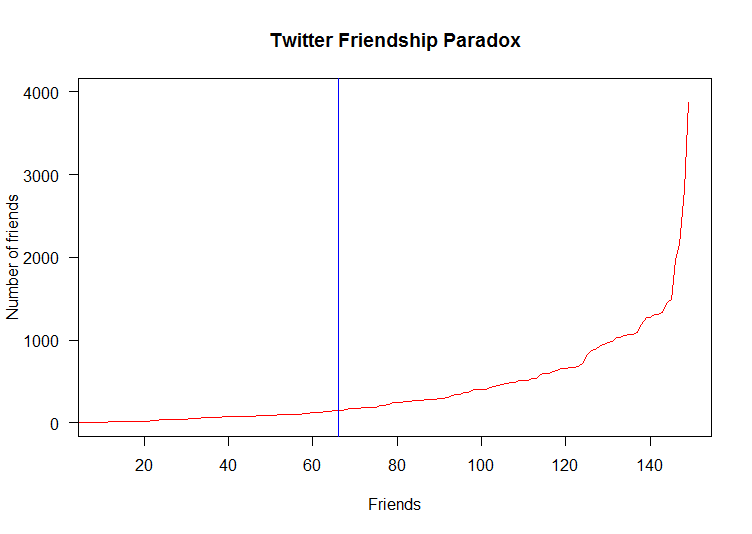
\includegraphics[scale=0.7]{../twitter/curveScatterPlot}
\centering
\caption{Twitter friendship paradox}

\label{scaled-scatterplot}
\end{figure}

\subsection{Calculations}
The mean, median, and standard deviation are calculated by using mosaic on ``R''.
\subsubsection{Executed the following commands}
install.packages("mosaic")\\*
install.packages("lattice")\\*
require(mosaic)\\*
favstats(finalSorted\$friendFriendsCount)
\subsubsection{Results}
Mean              : 405.5772\\*
Median            : 191\\*
Standard Deviation: 547.0392\\*
\newpage


%-----------------------End Question 1----------------------------

%------------------------------------------------------------------
%Question 2 (Facebook)
%------------------------------------------------------------------
\section{Question 2: Facebook Friendship Paradox}
Explore the friendship paradox for Facebook account.
%-----------------------Approach----------------------------------
\subsection{Approach}
I didn't follow any approach just used Alex's code. With the knowledge I got from my friends that by using Facebook API keys one cannot extract the number of friends due to several privacy issues.So, I used Alex's program to extract the friends. There was an issue when I try to use the program, the program never get's connected to my Facebook profile because of some security reason and was unable to find what is the reason.So,I used one of my friend's(Ramesh Govindarajulu) account and extracted the data.I did a very small change in the program like the way it was writing to the file.And used my sorting program to sort the friends count and saved results to a file and that it is loaded into ``R'' and the graphs are generated.

\newpage
%-----------------------Source Code---------------------------
\subsection{Source Code}

\subsubsection{searchFriends.py}
\lstinputlisting[breaklines=True,language=Python]{../facebook/seleniumScrapePB.py}

\subsubsection{sortingCommand.txt}
\lstinputlisting[breaklines=True,language=Python]{../facebook/sortCommand.txt}
\newpage
\subsubsection{sortFriends.py}
\lstinputlisting[breaklines=True,language=Python]{../twitter/sortFriends.py}
\newpage
%-----------------------Input Section---------------------------
\subsection{Input}
To accomplish the task ``Ramesh Govindarajulu'' facebook account is used.

%-----------------------Output Section---------------------------
\subsection{Output Files}

\subsubsection{facebookFriendFriendsCountTuples.txt}
The file contains the ``Ramesh Govindarajulu'' friends name and the count of their friends.
\lstinputlisting[breaklines=True]{../facebook/faceRawfordoc.txt}

\subsubsection{sortFacebook.txt}
Sorting the friends based on the number of friends.
\lstinputlisting[breaklines=True]{../facebook/sortFacebookfordoc.txt}

\subsubsection{finalSortedFacebook.txt}
The file contains the friend ID and number of friends for each friend.
\lstinputlisting[breaklines=True]{../facebook/finalSortedFacebookfordoc.txt}

\subsubsection{numberNameCountFb.txt}
This is a log file which contains ID given to each friend, count of friend friends, and  user name.
\lstinputlisting[breaklines=True]{../facebook/numberNameCountFbfordoc.txt}
\newpage


\subsection{Scatterplot}
\subsubsection{Code to generate the Scatterplot scatterCommands.txt}
\lstinputlisting[breaklines=True]{../facebook/scatterplotCommands.txt}
\subsubsection{Description of graph}

\begin{figure}[ht]
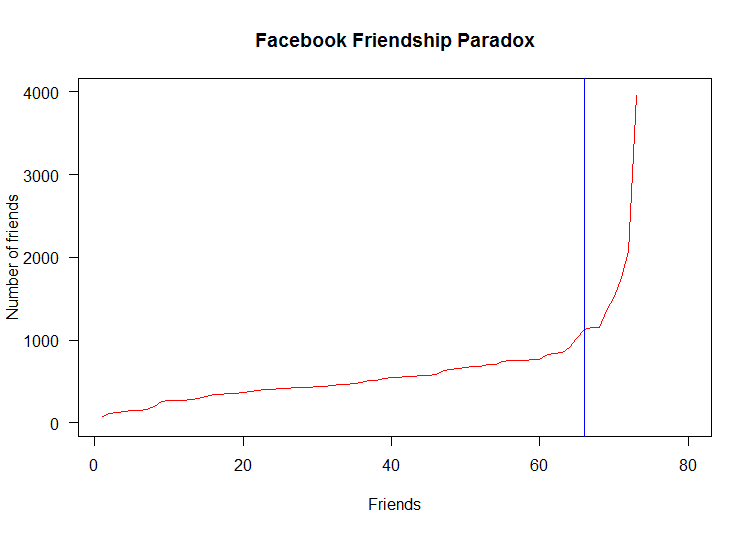
\includegraphics[scale=0.7]{../facebook/scatterplot1}
\centering
\caption{Facebook friendship paradox}
\label{intial-scatterplot}
\end{figure}


\begin{figure}[ht]
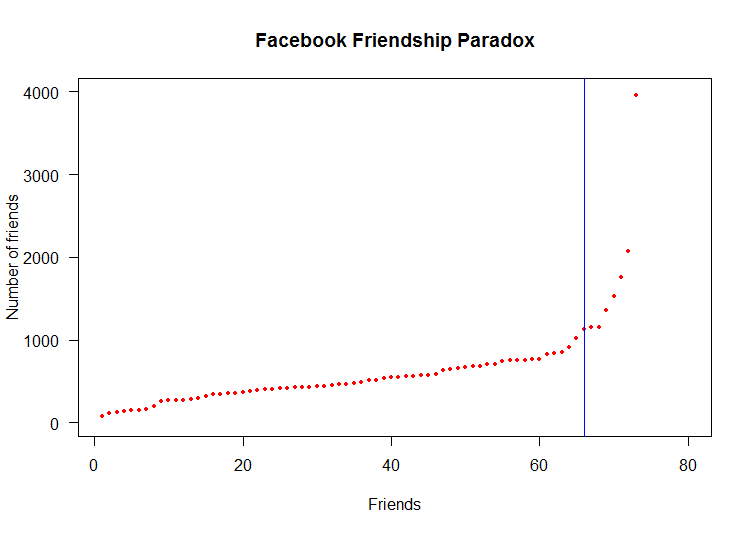
\includegraphics[scale=0.7]{../facebook/scatterplot2}
\centering
\caption{Facebook friendship paradox}
\label{scaled-scatterplot}
\end{figure}
\newpage
\subsection{Calculations}
The mean, median, and standard deviation are calculated by using mosaic on R.
\subsubsection{Executed the following commands}
install.packages("mosaic")\\*
install.packages("lattice")\\*
require(mosaic)\\*
favstats(finalSorted\$friendFriendsCount)
\subsubsection{Results}
Mean              : 626.8904\\*
Median            : 510\\*
Standard Deviation: 538.8189\\*
\newpage

%------------------------------------------------------------------
%Bibilography
%------------------------------------------------------------------
\bibliographystyle{plain}
\bibliography{A5_report}
\cite{*}
\end{document}